\documentclass[11pt, a4paper]{scrreprt}

\usepackage[ngerman]{babel}
\usepackage[utf8]{inputenc}
\usepackage[T1]{fontenc}
\usepackage[sfdefault, light]{roboto}
\usepackage[all]{nowidow}
\usepackage{graphicx, curves, float, rotating}
\usepackage[usenames, dvipsnames, svgnames, table]{xcolor}
\usepackage{mathtools, amssymb}
\usepackage[sort, numbers]{natbib}
\usepackage[position=bottom, labelfont=sf]{caption}
\usepackage[hidelinks]{hyperref}
\usepackage{pgfgantt}

% Page margins:
\usepackage[
	top=25mm,
	bottom=30mm,
	left=25mm,
	right=25mm
]{geometry}

% Colors:
\definecolor{blau}{HTML}{355FB3}
\definecolor{rot}{HTML}{B33535}
\definecolor{gruen}{HTML}{3BB335}
\definecolor{hellblau}{HTML}{8ea7d7}

% Fonts:
\renewcommand{\rmdefault}{ppl}
\renewcommand{\baselinestretch}{1.2}
\renewcommand{\familydefault}{\rmdefault}

\addtokomafont{subject}{\sffamily\mdseries}
\addtokomafont{title}{\usekomafont{subject}\color{blau}}
\addtokomafont{author}{\usekomafont{subject}}
\addtokomafont{date}{\usekomafont{subject}\normalsize}
\addtokomafont{publishers}{\usekomafont{subject}}
\addtokomafont{titlehead}{\raggedleft\sffamily\mdseries\small\textit}

\addtokomafont{pagenumber}{\sffamily\mdseries}

\addtokomafont{section}{\usekomafont{title}}
\addtokomafont{subsection}{\sffamily\mdseries}

% Change References title style:
\renewcommand{\bibsection}{\section*{\bibname}}

% Remove chapter numbers from section numbering:
\renewcommand*\thesection{\arabic{section}}
\renewcommand*\thefigure{\arabic{figure}}

% Disable paragraph indent:
\setlength{\parindent}{0pt}

\begin{document}

\section*{Beispiel}

\begin{figure}[h]
	\centering
	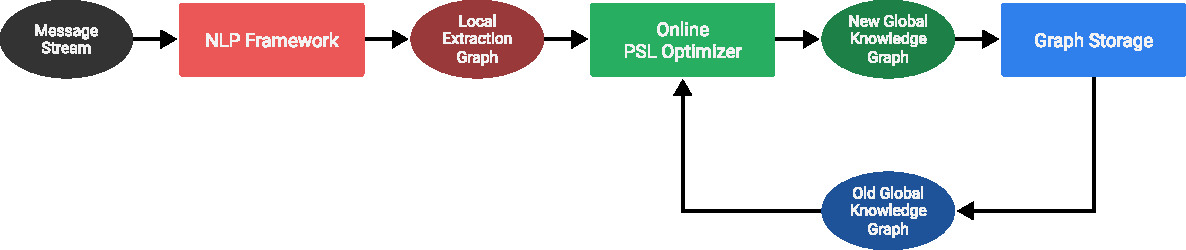
\includegraphics[width=\linewidth]{assets/overview}
	\caption{Vorläufiges grobes Strukturdiagramm des Verfahrens}\label{fig:overview}
\end{figure}

Der vorgestellte Ansatz zur Wissensgraphkonstruktion lässt sich in zwei Hauptschritte unterteilen.
Diese beiden Schritte werden beim Eintreffen einer Nachricht sequentiell ausgeführt.
Im ersten Schritt wird mittels eines NLP-Systems ein lokaler Konzeptgraph extrahiert, der strukturiert den Inhalt der eingetroffenen Nachricht repräsentiert.
Im zweiten Schritt wird dieser lokale Konzeptgraph dann in den bereits existierenden Wissensgraphen eingefügt.
Mittels eines PSL-Systems werden dann Beziehungen zwischen dem eingefügten Graphen und dem bestehenden Graphen ermittelt.\\

Zur Veranschaulichung dieses Verfahrens folgt ein Beispiel.
Gegeben sei folgende Nachricht, die am 12.06.2017 von Alice an Bob gesendet wurde:
\emph{``I don't think I saw you yesterday.''}

\begin{figure}[h]
	\centering
	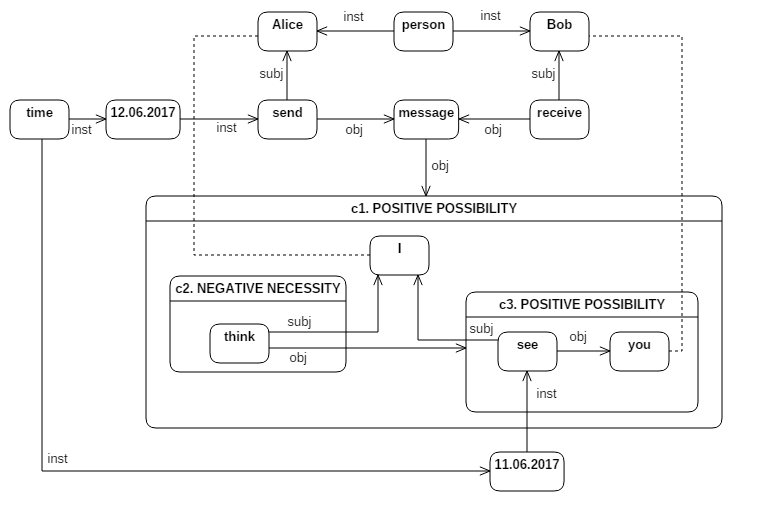
\includegraphics[width=0.8\linewidth]{assets/exampleExtractionGraph}
	\caption{Lokaler Konzeptgraph der obigen Nachricht}\label{fig:exampleExtractionGraph}
\end{figure}

Da Konzeptgraphen ein formales Kalkül von der Mächtigkeit einer Prädikatenlogik erster Ordnung sind, lässt sich dieser Graph auch durch folgenden äquivalenten Ausdruck beschreiben:
\begin{align*}
	\exists \,& person, time, alice, bob, msg, send, receive, d_1, d_2, c_1:\\
	& label(person, \text{`person'}) \land label(time, \text{`time'}) \land label(alice, \text{`Alice'}) \land label(bob, \text{`Bob'})\\
	& \land label(msg, \text{`message'}) \land label(send, \text{`send'}) \land label(receive, \text{`receive'})\\
	& \land label(d_1, 12.06.2017) \land label(d_2, 11.06.2017) \land class(time) \land class(person) \land class(d_1)\\
	& \land class(d_2) \land obj(person, alice) \land obj(person, bob) \land obj(time, d_1) \land obj(time, d_2)\\
	& \land obj(d_1, send) \land obj(send, msg) \land obj(receive, msg) \land subj(send, alice)\\
	& \land subj(receive, bob) \land obj(msg, c_1)\\
	& \begin{aligned}
		\land \,(&real(c_1) \leftrightarrow \exists \,c_3, i: label(i, \text{`I'}) \land i = alice\\
		& \land (\lnot\exists \,think: label(think, \text{`think'}) \land subj(think, i) \land obj(think, c_3))\\
		& \begin{aligned}
			\land \,(&real(c_3) \leftrightarrow \exists \,see, you: \land label(see, \text{`see'}) \land label(you, \text{`you'}) \land you = bob\\
			& \land obj(see, you) \land obj(d_2, see) \land subj(see, i)))
		\end{aligned}
	\end{aligned}
\end{align*}

Da Sprache nicht notwendigerweise Wahrheiten beschreibt, wird allen aus einer Nachricht extrahierten Konzepten eine Existenz- bzw.\ Nonexistenz-Aussage, sowie eine modale Notwendigkeit bzw. Möglichkeit zugeordnet.
Diese Zuordnung erfolgt mittels der Einordnung aller Konzepte in einen Kontextbaum.
Wurzelkonzepte, die außerhalb eines Kontextes stehen werden per Definition als notwendigerweise existent angenommen.
Im Beispiel sind u.~a.\  \(alice\), \(bob\) und \(msg\) Wurzelkonzepte.\\

Die Nachricht \(msg\) führt im Beispiel nun einen möglicherweise existenten Kontext \(c_1\) ein.
Alle Konzepte innerhalb eines möglichen Kontextes sind höchstens so real, wie dieser Kontext.
Die Realität von \(c_1\) hängt primär von der Interpretation des einleitenden Konzeptes \(msg\) ab, d.~h.\ inwiefern der Inhalt von \(msg\) der Realität entspricht.
Um dies abschätzen zu können, ist zusätzliches domänenspezifisches Wissen erforderlich, welches aus dem kompletten Wissensgraphen stammen muss;
da in der NLP-Phase Nachrichten isoliert betrachtet werden, kann eine Abwägung der Realität von extrahierten Möglichkeiten also erst in der PSL-Phase erfolgen.\\

Im Beispiel enthält \(c_1\) einen notwendigerweise nonexistenten Kontext \(c_2\).
Dies bedeutet, dass \(think\) nicht existiert gdw.\  \(c_1\) real ist.
\(think\) führt nun wiederum einen möglicherweise existenten Kontext \(c_3\) ein.
Um die Realität von \(c_3\) abzuschätzen ist, wie schon bei \(c_1\), domänenspezifisches Wissen aus dem kompletten Wissesgraphen erforderlich;
konkrekt muss ermittelt werden, welche Implikationen die Nonexistenz des Denkens von \(c_3\) auf die Realität von \(c_3\) hat.

\begin{figure}[H]
	\centering
	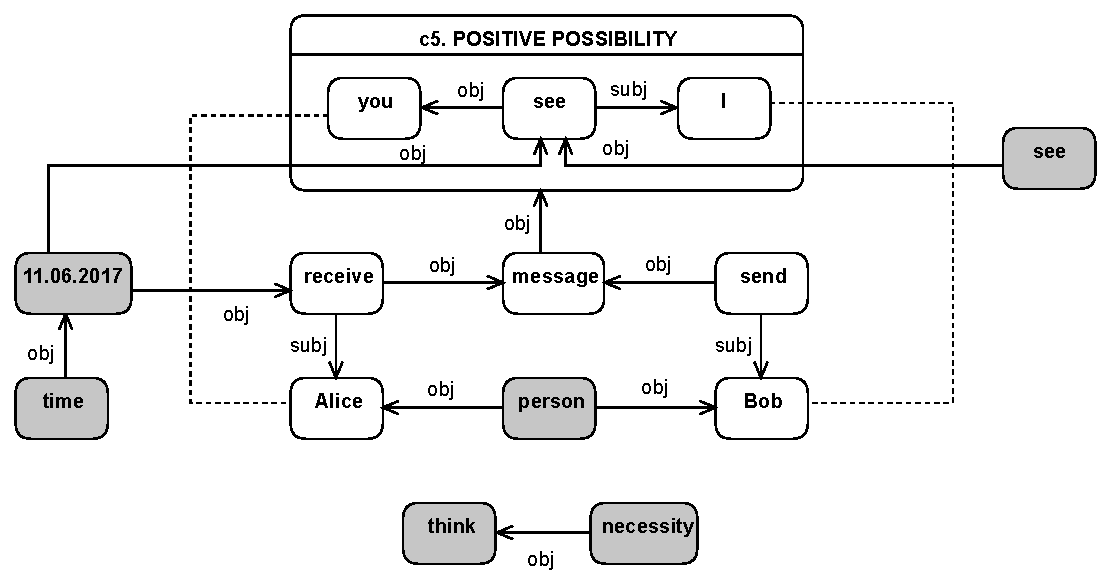
\includegraphics[width=0.8\linewidth]{assets/exampleOldKnowledgeGraph}
	\caption{Wissensgraph vor Einfügen der Nachricht}\label{fig:exampleOldKnowledgeGraph}
\end{figure}

Abb.~\ref{fig:exampleOldKnowledgeGraph} zeigt den kompletten Wissensgraphen vor Einfügen des Extraktionsgraphen aus Abb.~\ref{fig:exampleExtractionGraph}.
In diesem Beispiel wird davon ausgegangen, dass Bob zuvor am 11.06.2017 eine Nachricht an Alice mit dem Inhalt \emph{``I saw you today.''}  geschickt hat.
Außerdem wird davon ausgegangen, dass im Wissensgraphen bereits Informationen über das Konzept des Denkens vorhanden sind;
konkret wird durch die Verknüpfung mit \(necessity\) abgebildet, dass das Denken als Notwendigkeit verstanden werden kann, d.~h.\ dass für jede Aussage gilt, dass sie entweder gedacht wird oder ihr Gegenteil gedacht wird.
Diese Interpretation ist selbstverständlich nur eine von vielen;
sie wurde gewählt, da sie oftmals zutrifft und das Modell dabei einfach hält.\\

\begin{figure}[h]
	\centering
	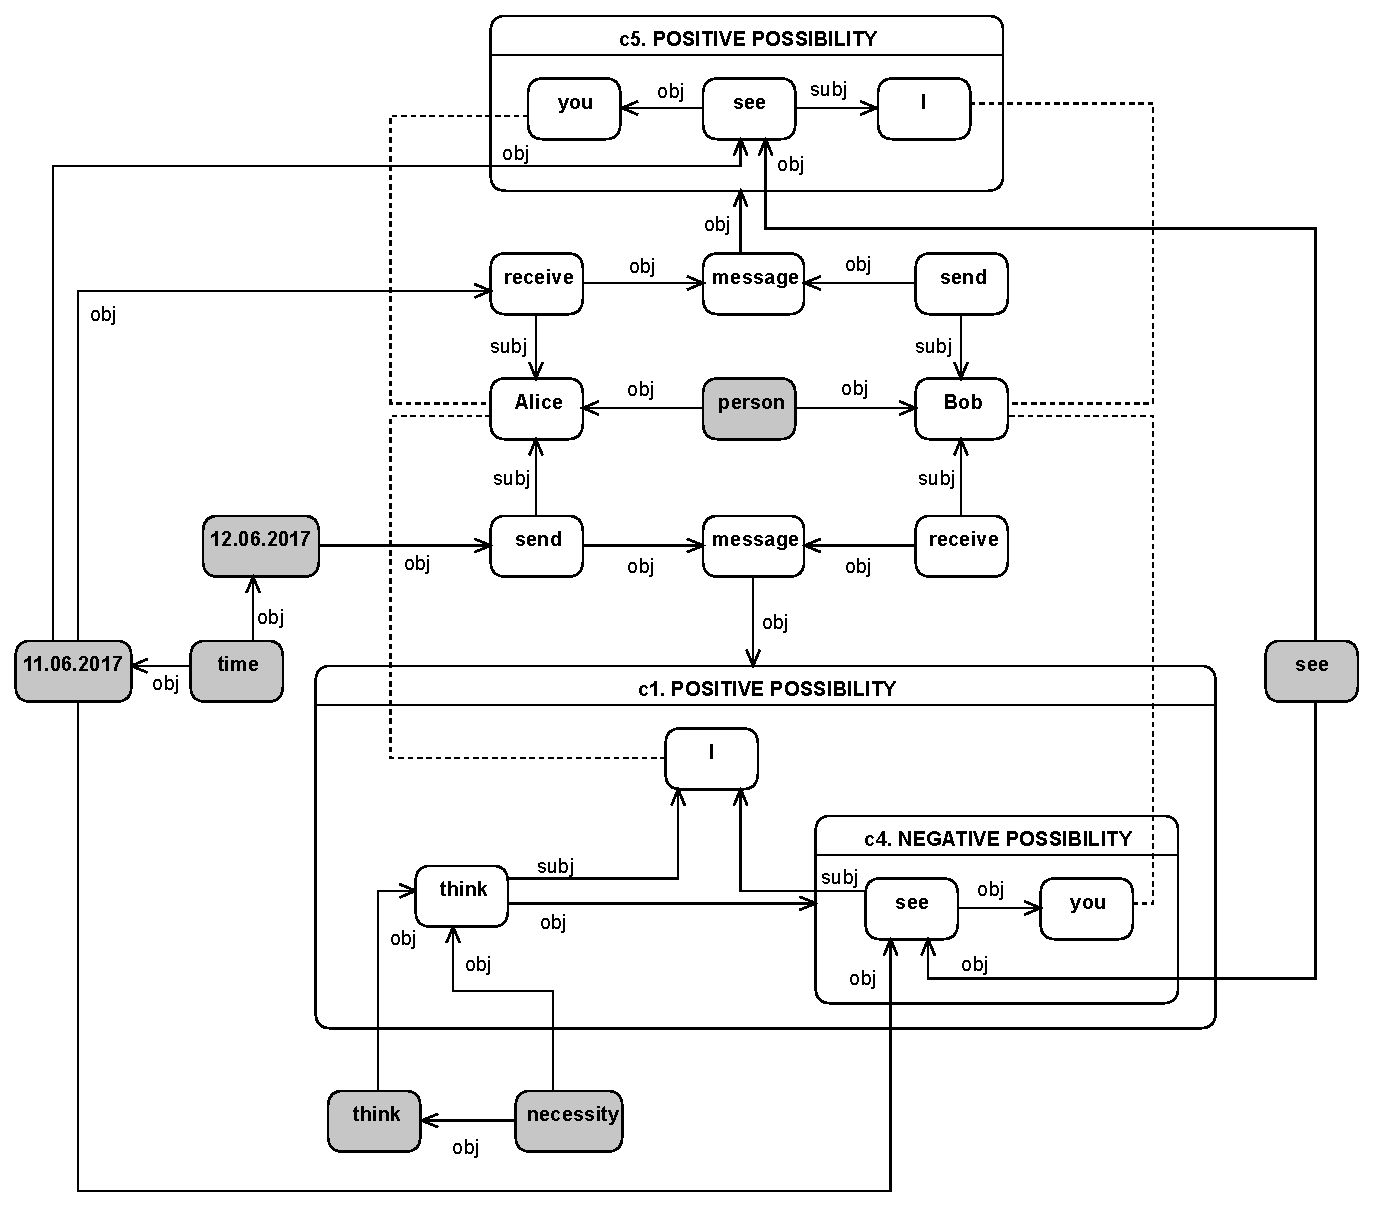
\includegraphics[width=0.8\linewidth]{assets/exampleKnowledgeGraph}
	\caption{Wissensgraph nach Einfügen der Nachricht}\label{fig:exampleKnowledgeGraph}
\end{figure}

Das Einfügen der Nachricht erfolgt im Rahmen der PSL-Phase (siehe Abb.~\ref{fig:exampleKnowledgeGraph}).
Im ersten Schritt wird der aktuelle Wissensgraph und der einzufügende Extraktionsgraph vereinigt.
Knoten mit gleicher Identität werden dabei durch Vereinigen der Inzidenzkantenmengen zusammengefasst, dies ist geschehen bei \(time\), \(person\), \(alice\), \(bob\) und \(11.06.2017\).\\

Anschließend erfolgt eine PSL-Optimierung, während der neue Kanten zwischen eingefügten und bestehenden Knoten entstehen.
Eine der grundlegendsten PSL-Regeln ist das Erkennen des Auftretens bekannter Konzepte mittels Label-Ähnlichkeit.
\[w_1:\ similar(A, B) \land class(A) \rightarrow obj(A, B)\]

Mit dieser Regel lässt sich z.~B.\ das globale Konzept des Denkens mit der lokalen Repräsentation des Denkens in \(c_1\) verknüpfen.
\(similar(A, B)\) könnte hierbei z.~B.\ über die Levenshtein-Distanz der Label von \(A\) und \(B\) definiert werden.
Da PSL eine probabilistische Logik ist, werden während der PSL-Phase alle logischen Aussagen als Wahrscheinlichkeiten \(\in [0, 1]\) interpretiert.
Dementsprechend sind PSL-Regeln nicht als Forderungen zu verstehen, die unbedingt eingehalten werden müssen, sondern eher als Indikatoren, die die Wahrscheinlichkeiten der implizierten Atome heben oder senken.\\

Um die Notwendigkeit der lokalen Denken-Repräsentation aus der Notwendigkeit des globalen Konzeptes zu folgern, wird eine weitere grundlegende PSL-Regel zur Beschreibung der Transitivität der \(obj\)-Relation benutzt:
\[w_2:\ class(A) \land class(B) \land obj(A, B) \land obj(B, C) \rightarrow obj(A, C)\]

Zur Erklärung des Wissensgraphen aus Abb.~\ref{fig:exampleKnowledgeGraph} ist nun noch eine weitere Regel notwendig.
Über die Relation des lokalen Nicht-Denkens zum \(necessity\)-Konzept, wurde gefolgert, dass ein lokales Denken des Gegenteils von \(c_3\) existiert.
Für diese Schlussfolgerung muss das \(necessity\)-Konzept eine Bedeutung erhalten.
Idealerweise sollte diese Bedeutung als Teil des Wissensgraphen kodiert sein und mittels weiterer grundlegender PSL-Regeln zu der gewünschten Interpretation führen.
Da PSL-Regeln allerdings weniger mächtig als aussagenlogische Ausdrücke und somit als prädikatenlogische Ausdrücke sind, ist dies nicht ohne Weiteres möglich.
Um das PSL-System einfach zu halten, werden daher stattdessen domänenspezifische Regeln eingeführt.
\[w_3: class(N) \land label(N, \text{`necessity'}) \land obj(N, A) \land neg(A) \land obj(A, C) \land possib(C) \rightarrow \lnot \, real(C)\]

In einem vollständigen PSL-System existieren selbstverständlich noch andere Regeln und die drei genannten sind primär als Beispiel zu verstehen.
Die genaue zu verwendende Regelmenge muss noch spezifiziert werden.
Einen Ausgangspunkt für die Wahl der Regeln bietet dieses Paper: \url{https://arxiv.org/pdf/1607.00992v1.pdf}.

\end{document}
